\documentclass[twoside]{article}
\usepackage{amsgen,amsmath,amstext,amsbsy,amsopn,amssymb,color}
\usepackage{graphicx}
\usepackage{epsfig}

\setlength{\oddsidemargin}{0.1 in} \setlength{\evensidemargin}{-0.1
in} \setlength{\topmargin}{-0.6 in} \setlength{\textwidth}{6.5 in}
\setlength{\textheight}{10.5 in} \setlength{\headsep}{0.1 in}
\setlength{\parindent}{0 in} \setlength{\parskip}{0.1 in}

\newcommand{\red}{\textcolor{red}}

\newcommand{\homework}[2]{
   \pagestyle{myheadings}
   \thispagestyle{plain}
   \newpage
   \setcounter{page}{1}
   \noindent
   \begin{center}
   \framebox{
      \vbox{\vspace{2mm}
       \hbox to 6.28in { {\bf Math 4720:~Statistical Methods \hfill} }
       \vspace{6mm}
       \hbox to 6.28in { {\Large \hfill #1 (#2)  \hfill} }
       \vspace{6mm}
      \vspace{2mm}}
   }
   \end{center}
   \markboth{#1}{#1}
   \vspace*{4mm}
}

\newcommand{\bbF}{\mathbb{F}}
\newcommand{\bbX}{\mathbb{X}}
\newcommand{\bI}{\mathbf{I}}
\newcommand{\bX}{\mathbf{X}}
\newcommand{\bY}{\mathbf{Y}}
\newcommand{\bepsilon}{\boldsymbol{\epsilon}}
\newcommand{\balpha}{\boldsymbol{\alpha}}
\newcommand{\bbeta}{\boldsymbol{\beta}}
\newcommand{\0}{\mathbf{0}}

\begin{document}

\homework{$8^{th}$ Week Summary}{3/6/25}
\vspace{-0.4 in}
\begin{figure}[h]
\begin{center}
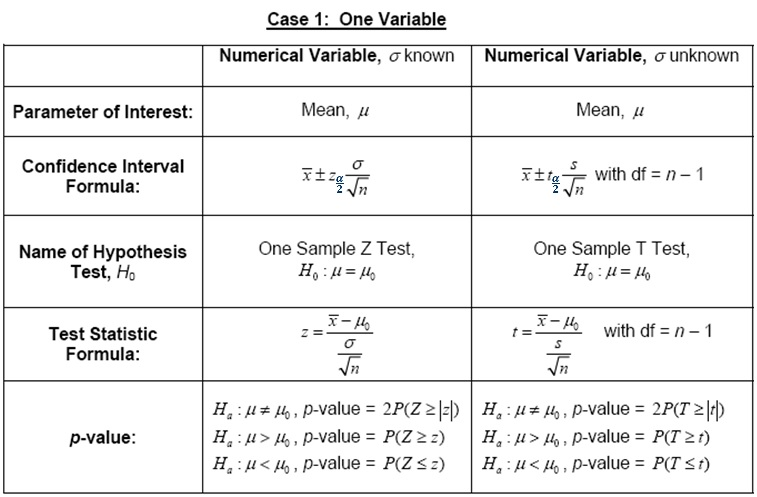
\includegraphics[angle=0, width=10.5 cm] {HT_1.jpg}
\end{center}
\end{figure}
\vspace{-0.3 in}
\begin{figure}[h]
\begin{center}
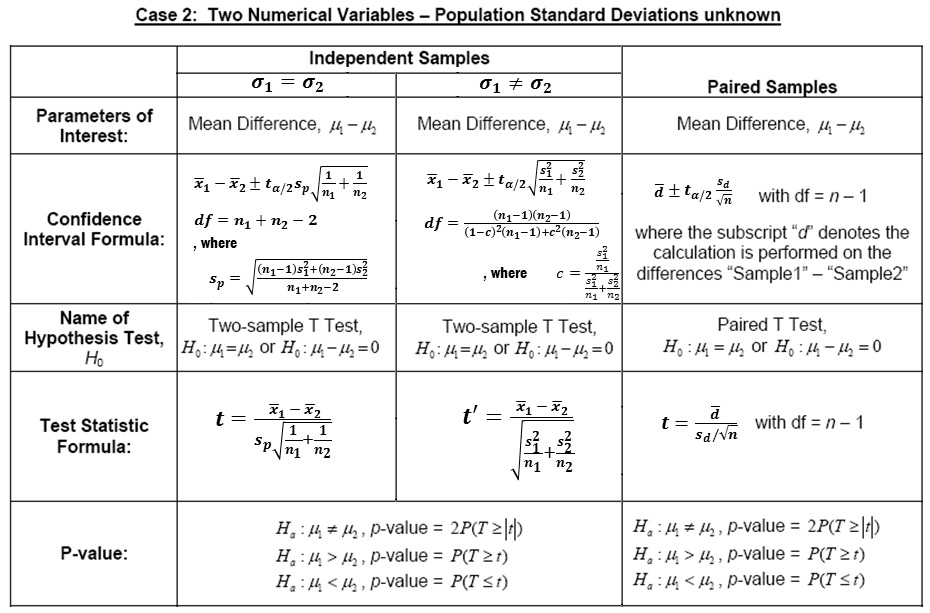
\includegraphics[angle=0, width=16 cm] {HT_3.jpg}
\end{center}
\end{figure}
\begin{itemize}
\vspace{-0.3 in}
\item \textbf{Power analysis} (Sample size determination):
\subitem \textbf{Independent Samples}:
\subsubitem For one sided alternative test ($H_a:\mu_1>\mu_2$ or $H_a:\mu_1<\mu_2$ ): $n=\dfrac{2\sigma^2(z_\alpha+z_\beta)^2}{\Delta^2}$
\subsubitem For two sided alternative test ($H_a:\mu_1 \neq \mu_2$): $n=\dfrac{2\sigma^2(z_{\alpha/2}+z_\beta)^2}{\Delta^2}$
\subitem \textbf{Paired Data}:
\subsubitem For one sided alternative test ($H_a:\mu_d>0$ or $H_a:\mu_d<0$ ): $n=\dfrac{\sigma_d^2(z_\alpha+z_\beta)^2}{\Delta^2}$
\subsubitem For two sided alternative test ($H_a:\mu_d \neq 0$): $n=\dfrac{\sigma_d^2(z_{\alpha/2}+z_\beta)^2}{\Delta^2}$
\end{itemize}

\newpage
\vspace{1.3 in}
\begin{itemize}
\item \textbf{NON-PARAMETRIC TESTS}\dotfill
\item Test for the population median M:
\subitem SIGN TEST:
\subsubitem Test Statistics: B = \# of data values $> m_0$
\subsubitem Minitab: Stat $\rightarrow$ Nonparametrics $\rightarrow$ 1-Sample Sign
\subsubitem R: \textsf{library("BSDA"); SIGN.test(dataset)}
\item Non-parametric TWO Independent Samples Test:
\subitem WILCOXON RANK-SUM TEST(MANN–WHITNEY U TEST)
\subsubitem Combine both the samples. Rank all values of the combined sample from lowest to the highest.
$$\textrm{T= sum of the ranks insample 1}$$
\subsubitem Minitab: Stat $\rightarrow$ Nonparametrics $\rightarrow$ Mann-Whitney
\subsubitem R: \textsf{wilcox.test(group1, group2)}
\item Non-parametric TWO Dependent Samples Test:
\subitem WILCOXON SIGNED-RANK TEST
\subsubitem Test Statistics: Rank the absolute values of the differences. $$\textrm{T= sum of the ranks of negative(positive) differences}$$
\subsubitem Minitab: For differences, Minitab: Stat $\rightarrow$ Nonparametrics $\rightarrow$ 1-Sample Wilcoxon
\subsubitem R: \textsf{wilcox.test(before, after, paired = T)}
\end{itemize}
\vspace{-.25in}\hrulefill\vspace{-.15in}
\end{document}


